\subsection{Safety} %Martina
\noindent In this section the safety aspect of the mechanical part in this project will be discussed. As safety is an important factor in any situation, especially when constructing an underwater vehicle, a safe system has been adapted in order to protect those who operate together with Naiad. Safety can always be improved, but in this project it has been taken as far as time has allowed and the safety which was already present when taking over the project has been further improved. 

	\subsubsection{Thruster safety nets}
\noindent The thrusters that are used for Naiad do originally not have safety nets covering the openings. This results in an increased risk of injury, e.g. by accidentally grabbing hold of the thrusters and placing one's fingers inside of the opening when manually maneuvering the underwater vehicle. It was therefore decided that safety nets should be designed and 3D-printed for mounting on the front and rear openings of the thrusters. 

Several designs were 3D-printed and tested, with varying thickness and width of the net structure. The design which finally was used can be seen in fig. \ref{heej}. However, after a couple of underwater tests it was discovered that some of the safety nets had broken and seemed fragile so the choice of material was questioned. The safety nets are printed in Acrylonitrile butadiene styrene (ABS) plastic, which becomes more fragile when exposed to UV-light, but there should be no major harm to the material by exposing it to water. Then, it was thought that the breakage could have been due to the chlorine in the water. This was tested by adding chlorine to a pot of water and letting a safety net lay in the chlorine mixed water for about a week. There were no major changes to the piece. With this in mind, the safety nets most likely broke because they were too weak in the construction or they were pressed onto when being handled.

The design of the safety nets was changed after this discovery and the new design, which can be seen in fig. \ref{heeej}, includes a locking mechanism which is intended to hold the thruster cap in place much better and remove the need of having a nut on the screws to secure the safety nets to the thrusters. The first prototype of the nets was slightly too tight, resulting in that the net stuck to the thruster without the need of any screws at all. It was decided that this method worked well and was therefore adapted for the time being.  

This time the safety nets were printed in polylactide (PLA) plastic instead of ABS. PLA is supposed to be more fragile to water, but a piece of PLA was tested in the chlorine water at the same time as the ABS and, like the ABS, the PLA did not undergo any major changes.

\begin{figure}[!ht]
	\begin{center}
		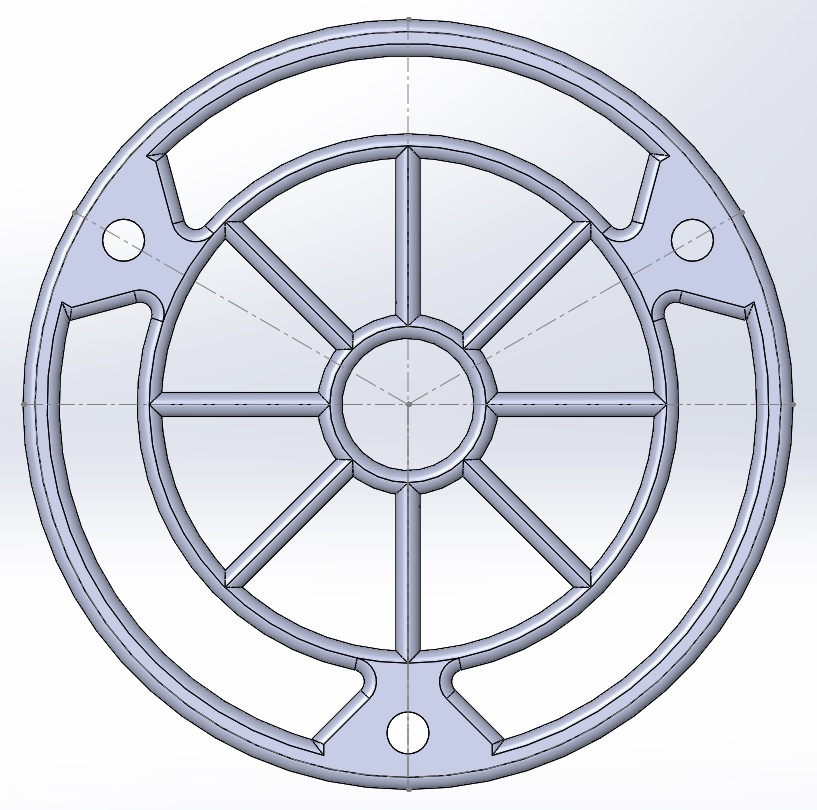
\includegraphics[width=80mm]{./Images/Mechanics/Safety_Net.jpg}
		\caption{The safety net used during most of the project.}
		\label{heej}
	\end{center}
\end{figure}

\begin{figure}[!ht]
	\begin{center}
		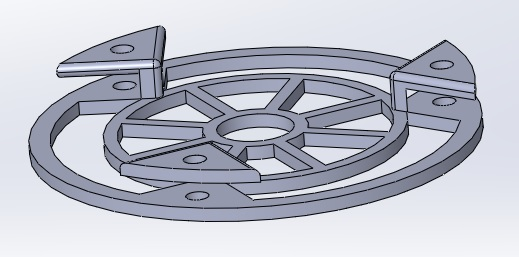
\includegraphics[width=80mm]{./Images/Mechanics/Safety_Net_With_Addon.jpg}
		\caption{The latest safety net with locking device.}
		\label{heeej}
	\end{center}
\end{figure}

	
	\subsubsection{Kill switch and mission switch}
\noindent The kill and mission switches add safety to the system. In case of emergency, the kill switch will shut down the motors when being removed from the hull. The mission switch makes sure that Naiad does not start a mission without the switch being activated. If this was not the case, it could lead to unexpected movement and as a result cause injuries on people around Naiad or damages to Naiad itself. 

The kill and mission switches were redesigned as the previous version turned out not to work with the placement of the magnets. Depending on the size of the magnets, they were either too weak to interact with the hall sensor or interfering with the hall sensor too much as the magnets for attaching the switches to the hull and the ones for reacting with the hall sensor were too close to each other.  
